\documentclass[a4paper,12pt]{article}
\usepackage{ctex}
\usepackage{amsmath}
\usepackage{graphicx}
\usepackage{geometry}
\usepackage{diagbox}
\usepackage{multirow}
\usepackage{hyperref}
\usepackage{float}
\usepackage{tikz}
\usepackage{subcaption}
\usepackage{csvsimple}
\usepackage{array}
\usepackage{tabularx}
\usetikzlibrary{arrows.meta,positioning}
\newcolumntype{Y}{>{\centering\arraybackslash}X}
\geometry{left=2.5cm,right=2.5cm,top=2.5cm,bottom=2.5cm}
\graphicspath{{figures/}{results/}}

\begin{document}
\begin{titlepage}
    \centering
    \vfill
    {\zihao{0}\bfseries 电子测试与实验技术\\[0.6em]实验报告\par}
    \vfill
    \vfill

    \begin{minipage}{0.72\textwidth}
        \zihao{-2}
        学\quad\quad 院：\underline{\makebox[7.5cm][l]{光学与电子信息学院}}\\[1.6em]
        班\quad\quad 级：\underline{\makebox[7.5cm][l]{光电信息科学与工程202409班}}\\[1.6em]
        姓\quad\quad 名：\underline{\makebox[7.5cm][l]{陈\quad 恪\quad 瑾}}\\[1.6em]
        学\quad\quad 号：\underline{\makebox[7.5cm][l]{U 2 0 2 4 1 3 9 2 5}}\\[1.6em]
        实验时间：\underline{\makebox[7.5cm][l]{2026 年 05 月 14 日}}
    \end{minipage}

    \vfill
    \vfill
\end{titlepage}

\setcounter{page}{1}

\section{实验名称}
集成触发器及其应用（流水灯）

\section{实验目的}
\subsection{集成触发器功能验证}
\begin{enumerate}
    \item 了解 74HC74 触发器的逻辑功能及主要性能指标。
    \item 掌握集成触发器逻辑功能测试方法。
    \item 熟悉用双踪示波器观察并测量多路时序信号的方法。
\end{enumerate}

\subsection{流水灯设计与实现}
\begin{enumerate}
    \item 掌握用触发器构成同步可逆模 4 计数器的方法。
    \item 掌握用与非门实现 2-4 线译码器的方法。
    \item 掌握简单时序逻辑电路的安装、调试与故障排查流程。
    \item 理解计数器与译码器配合实现流水灯正转和反转的工作机理。
\end{enumerate}

\section{实验元器件}
\subsection{触发器功能验证}
\begin{table}[H]
\centering
\caption{触发器功能验证元器件}
\begin{tabular}{|c|c|c|}
\hline
类型 & 型号（参数） & 数量 \\
\hline
集成电路 & 74HC74 & 1片 \\
\hline
集成电路 & 74HC00 & 1片 \\
\hline
\end{tabular}
\end{table}

\subsection{流水灯设计与实现}
\begin{table}[H]
\centering
\caption{流水灯实验元器件}
\begin{tabular}{|c|c|c|}
\hline
类型 & 型号（参数） & 数量 \\
\hline
集成电路 & 74HC74 & 1片 \\
\hline
集成电路 & 74HC00 & 2片 \\
\hline
集成电路 & 74HC10 & 1片 \\
\hline
电阻 & 510$\Omega$ & 4只 \\
\hline
发光二极管 & 红/黄/绿（共4只） & 4只 \\
\hline
\end{tabular}
\end{table}

\section{实验原理及参考电路}
\subsection{触发器的逻辑功能及其相互转换}
典型触发器的特性方程如下表：

\begin{table}[H]
\centering
\renewcommand{\arraystretch}{1.4}
\begin{tabularx}{0.98\textwidth}{|c|Y|Y|Y|Y|}
\hline
类型 & JK触发器 & D触发器 & T触发器 & T'触发器 \\
\hline
特征方程 &
$Q^{n+1}=J\overline{Q^n}+\overline{K}Q^n$ &
$Q^{n+1}=D$ &
$Q^{n+1}=T\oplus Q^n$ &
$Q^{n+1}=\overline{Q^n}$ \\
\hline
\end{tabularx}
\end{table}

触发器的转换方法如下表：

\begin{table}[H]
\centering
\renewcommand{\arraystretch}{1.4}
\begin{tabularx}{0.98\textwidth}{|c|Y|Y|Y|Y|}
\hline
\multirow{2}{*}{原触发器} & \multicolumn{4}{c|}{转换成} \\
\cline{2-5}
\multicolumn{1}{|c|}{} & T触发器 & T'触发器 & D触发器 & JK触发器 \\
\hline
D触发器 & $D=T\oplus Q^n$ & $D=\overline{Q^n}$ &  & $D=J\overline{Q^n}+\overline{K}Q^n$ \\
\hline
JK触发器 & $J=K=T$ & $J=K=1$ & $J=D,\ K=\overline{D}$ &  \\
\hline
\end{tabularx}
\end{table}

\subsection{用触发器设计简单的时序逻辑电路的一般步骤}
\begin{enumerate}
    \item 逻辑抽象，建立原始状态图和原始状态表；
    \item 状态化简，消除等价状态，确定最简状态个数；
    \item 状态分配，通常用二进制或格雷码进行状态编码，并确定触发器个数及类型；
    \item 求解输入方程、输出方程、状态转换方程；
    \item 检查自启动能力，如可以自启动则画出逻辑电路图；不能自启动则需要将陷入死循环的状态指向工作循环，再重复第四步。
\end{enumerate}

\subsection{流水灯设计原理}
\subsubsection{功能需求}
每次CP到来时只允许一只发光二极管亮，且各二极管轮流发光；

\subsubsection{整体框架}
流水灯逻辑部分由同步可逆计数器和2-4线译码器组成，如下图：

\begin{figure}[H]
    \centering
    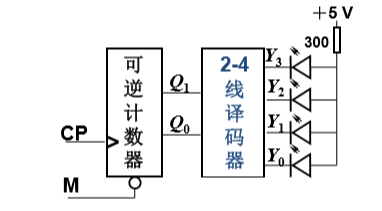
\includegraphics[width=0.62\textwidth]{figures/word_zhp_media/image1.png}
    \caption{流水灯逻辑部分总体框图}
\end{figure}

\subsubsection{实验要求}
用74HC74和与非门来实现电路，引出输入端M用于控制计数器计数模式，如：M=1为加法计数，M=0为减法计数。

\section{硬件实验内容}
\subsection{设计与推导}
\subsubsection{同步可逆模 4 计数器设计}
\textbf{① 状态转移图}

这是一个 4 状态摩尔型状态机，状态用两位二进制 $Q_1Q_0$ 编码：
$S_0:00,\ S_1:01,\ S_2:10,\ S_3:11$。输入变量为 $M$（控制端），边标注的是输入 $M$ 的取值。
当 $M=1$ 时，状态按 $S_0\rightarrow S_1\rightarrow S_2\rightarrow S_3\rightarrow S_0$ 循环（加计数）；
当 $M=0$ 时，状态按 $S_0\rightarrow S_3\rightarrow S_2\rightarrow S_1\rightarrow S_0$ 循环（减计数）。
因此该状态机是一个典型的模 4 可逆计数器。

\begin{figure}[H]
    \centering
    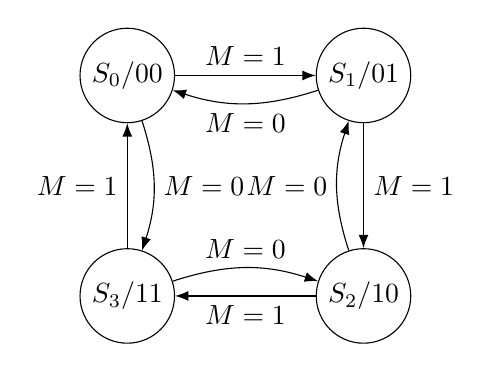
\begin{tikzpicture}[>=Latex, node distance=2.8cm]
        \tikzset{state/.style={draw, circle, minimum size=1.2cm, inner sep=1pt}}
        \node[state] (s0) at (0,1.8) {$S_0/00$};
        \node[state] (s1) at (3.0,1.8) {$S_1/01$};
        \node[state] (s2) at (3.0,-1.0) {$S_2/10$};
        \node[state] (s3) at (0,-1.0) {$S_3/11$};

        \draw[->] (s0) -- node[above] {$M=1$} (s1);
        \draw[->] (s1) -- node[right] {$M=1$} (s2);
        \draw[->] (s2) -- node[below] {$M=1$} (s3);
        \draw[->] (s3) -- node[left] {$M=1$} (s0);

        \draw[->] (s1) to[bend left=18] node[below] {$M=0$} (s0);
        \draw[->] (s2) to[bend left=18] node[left] {$M=0$} (s1);
        \draw[->] (s3) to[bend left=18] node[above] {$M=0$} (s2);
        \draw[->] (s0) to[bend left=18] node[right] {$M=0$} (s3);
    \end{tikzpicture}
    \caption{同步可逆模4计数器状态转移图}
\end{figure}

\textbf{② 状态转移表}

状态转移表将当前状态 $Q_1Q_0$、输入 $M$ 和次态 $Q_1^{n+1}Q_0^{n+1}$ 一一对应，作为后续逻辑化简依据：

\begin{table}[H]
\centering
\renewcommand{\arraystretch}{1.25}
\begin{tabular}{|c|c|c|c|c|c|}
\hline
状态 $S$ & $Q_1$ & $Q_0$ & $M$ & $Q_1^{n+1}$ & $Q_0^{n+1}$ \\
\hline
$S_0$ & 0 & 0 & 1 & 0 & 1 \\
\hline
$S_0$ & 0 & 0 & 0 & 1 & 1 \\
\hline
$S_1$ & 0 & 1 & 0 & 0 & 0 \\
\hline
$S_1$ & 0 & 1 & 1 & 1 & 0 \\
\hline
$S_2$ & 1 & 0 & 0 & 0 & 1 \\
\hline
$S_2$ & 1 & 0 & 1 & 1 & 1 \\
\hline
$S_3$ & 1 & 1 & 0 & 1 & 0 \\
\hline
$S_3$ & 1 & 1 & 1 & 0 & 0 \\
\hline
\end{tabular}
\end{table}

\textbf{③ 次态方程推导}

1) 对 $Q_1^{n+1}$ 作卡诺图化简可得：
\[
Q_1^{n+1}
=\overline{Q_1}\,\overline{Q_0}M
+Q_1\overline{Q_0}\,\overline{M}
+\overline{Q_1}Q_0\overline{M}
+Q_1Q_0M
=Q_1\oplus Q_0\oplus M.
\]
为便于与非门实现，可写为：
\[
Q_1^{n+1}
=\overline{
\overline{\overline{Q_1}\,\overline{Q_0}M}\cdot
\overline{Q_1\overline{Q_0}\,\overline{M}}\cdot
\overline{\overline{Q_1}Q_0\overline{M}}\cdot
\overline{Q_1Q_0M}
}.
\]

2) 对 $Q_0^{n+1}$ 作卡诺图化简得到最简式：
\[
Q_0^{n+1}=\overline{Q_0}.
\]
这说明低位触发器在每个时钟沿到来时翻转一次，符合二进制计数器低位特性。

\textbf{④ 驱动方程}

采用 D 触发器时，利用其特性方程 $Q^{n+1}=D$，可直接得到驱动方程：
\[
D_0=Q_0^{n+1}=\overline{Q_0},\qquad
D_1=Q_1^{n+1}.
\]
其中 $D_1$ 可取异或形式 $Q_1\oplus Q_0\oplus M$，也可取上式的与非门等效形式实现。

\textbf{④ 电路原理图}
根据上述推导结果，设计电路原理图如下：

\begin{figure}[H]
    \centering
    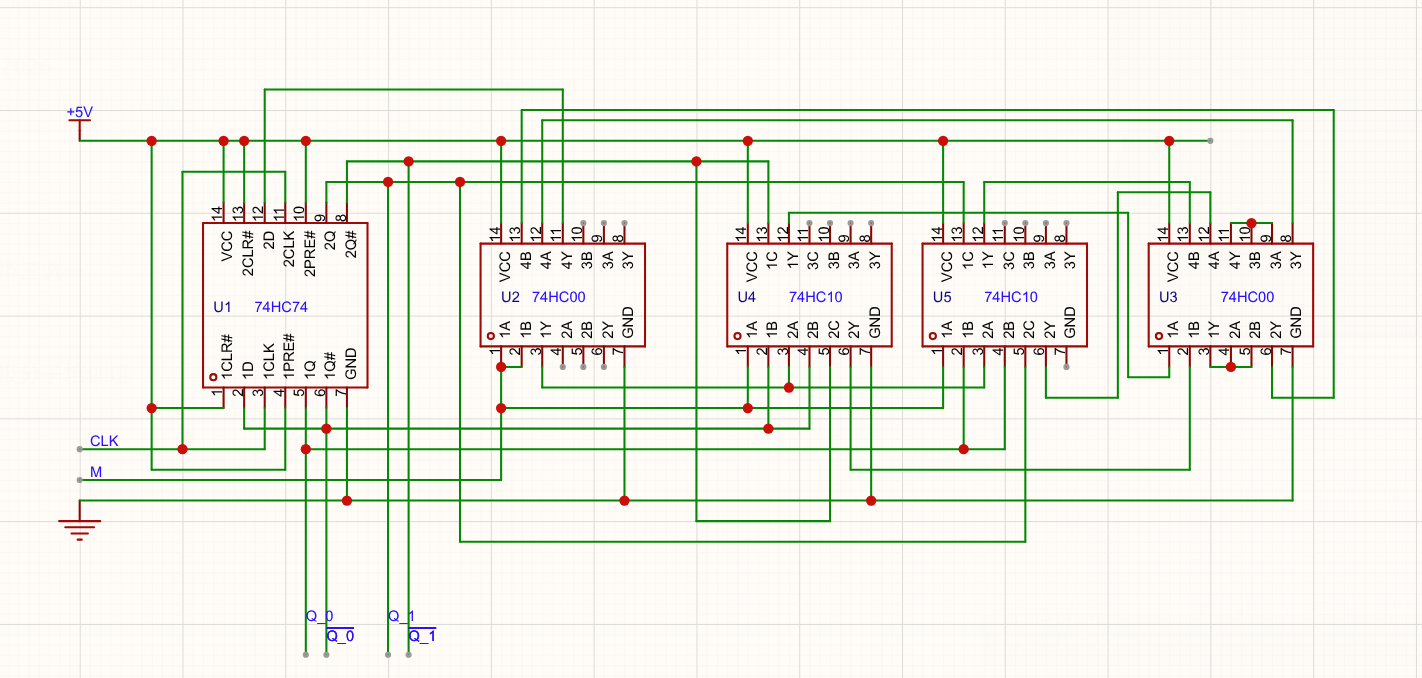
\includegraphics[width=0.95\textwidth]{figures/word_zhp_media/image.png}
    \caption{同步可逆模四计数器电路原理图}
\end{figure}

\subsubsection{2-4 线译码器设计}
\textbf{译码功能概述}

该模块输入为计数器状态位 $Q_1,Q_0$，输出为 $Y_0,Y_1,Y_2,Y_3$。本实验采用低电平有效输出，
即任一时刻仅有一路输出为 0，其余三路为 1，对应一路 LED 被选通点亮。

\textbf{真值表}

\begin{table}[H]
\centering
\renewcommand{\arraystretch}{1.25}
\begin{tabular}{|c|c|c|c|c|c|}
\hline
$Q_1$ & $Q_0$ & $Y_0$ & $Y_1$ & $Y_2$ & $Y_3$ \\
\hline
0 & 0 & 0 & 1 & 1 & 1 \\
\hline
0 & 1 & 1 & 0 & 1 & 1 \\
\hline
1 & 0 & 1 & 1 & 0 & 1 \\
\hline
1 & 1 & 1 & 1 & 1 & 0 \\
\hline
\end{tabular}
\end{table}

\textbf{输出方程推导}

由真值表先写出低有效输出的\textbf{原始逻辑方程（标准最小项和式）}：
\[
\begin{aligned}
Y_0&=\Sigma m(1,2,3)=\overline{Q_1}Q_0+Q_1\overline{Q_0}+Q_1Q_0,\\
Y_1&=\Sigma m(0,2,3)=\overline{Q_1}\,\overline{Q_0}+Q_1\overline{Q_0}+Q_1Q_0,\\
Y_2&=\Sigma m(0,1,3)=\overline{Q_1}\,\overline{Q_0}+\overline{Q_1}Q_0+Q_1Q_0,\\
Y_3&=\Sigma m(0,1,2)=\overline{Q_1}\,\overline{Q_0}+\overline{Q_1}Q_0+Q_1\overline{Q_0}.
\end{aligned}
\]
化简后可得：
\[
\begin{aligned}
Y_0&=Q_1+Q_0,\\
Y_1&=Q_1+\overline{Q_0},\\
Y_2&=\overline{Q_1}+Q_0,\\
Y_3&=\overline{Q_1}+\overline{Q_0}.
\end{aligned}
\]

\textbf{输出方程转换}

由于本实验仅限使用与非门实现，故需要对上述逻辑表达式变形，使逻辑表达式中的逻辑关系仅限为“与非”或“非”关系（“非”关系可以通过将与非门两个引脚同时接输入信号实现）：
\[
\begin{aligned}
Y_0&=\overline{\overline{Q_1}\,\overline{Q_0}},\\
Y_1&=\overline{\overline{Q_1}Q_0},\\
Y_2&=\overline{Q_1\overline{Q_0}},\\
Y_3&=\overline{Q_1Q_0}.
\end{aligned}
\]
上述四式均可直接由与非门结构实现。由于芯片资源限制，本实验不接使能端，仅实现 2 位输入到 4 路低有效输出的基本译码功能。

\textbf{电路原理图}

根据上述方程，2-4 线译码器与非门实现电路如下：

\begin{figure}[H]
    \centering
    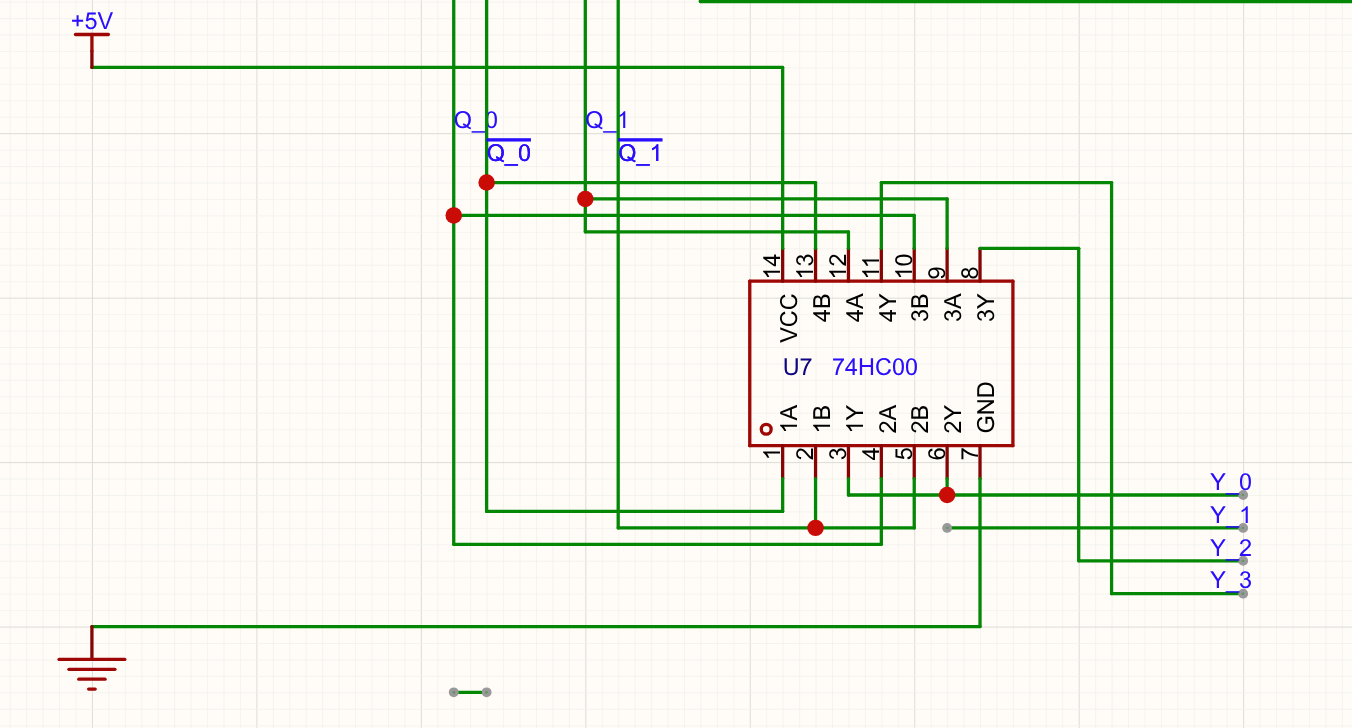
\includegraphics[width=0.82\textwidth]{figures/word_zhp_media/image0.png}
    \caption{2-4线译码器实现电路}
\end{figure}

\subsection{实验步骤}
\begin{enumerate}
    \item 输入 1Hz、5V 方波作为时钟，观察流水灯逻辑功能（$M=1$ 正转，$M=0$ 反转）。
    \item 输入 1kHz、5V 方波，测量并记录 $CP$、$M$、$Q_0$、$Q_1$ 等时序波形。
    \item 对照理论时序检查状态转移和译码输出是否一致。
\end{enumerate}

\section{硬件实验结果分析}
\subsection{实验现象}
上电后，电路能够按照预先设计的状态序列稳定运行。当 $M=1$ 时，计数器按 $S_0\rightarrow S_1\rightarrow S_2\rightarrow S_3\rightarrow S_0$ 依次循环，对应四个 LED 由左到右逐个点亮；当 $M=0$ 时，状态序列反向变化，对应 LED 由右到左逐个点亮。说明计数方向控制正确，流水灯的正转和反转功能均能实现。

\subsection{时序波形分析}
由示波器波形可知，$CLK$ 为外加时钟信号，$Q_0$ 在每个时钟上升沿翻转一次，因此其频率为时钟信号的二分频；$Q_1$ 只在两个完整计数周期后翻转一次，因此其频率为时钟信号的四分频。$Y_0\sim Y_3$ 为译码器输出，在任一时刻仅有一路输出为低电平，与当前状态一一对应，因此四个 LED 能按状态顺序轮流点亮。改变 $M$ 后，$Q_1,Q_0$ 的翻转顺序随状态方向同步改变，但分频关系和译码规律保持不变，说明同步可逆模 4 计数器及其译码部分均工作正常。

使用计算机绘图软件绘制示波器捕获的时序波形，结果如下：
\begin{figure}[H]
    \centering
    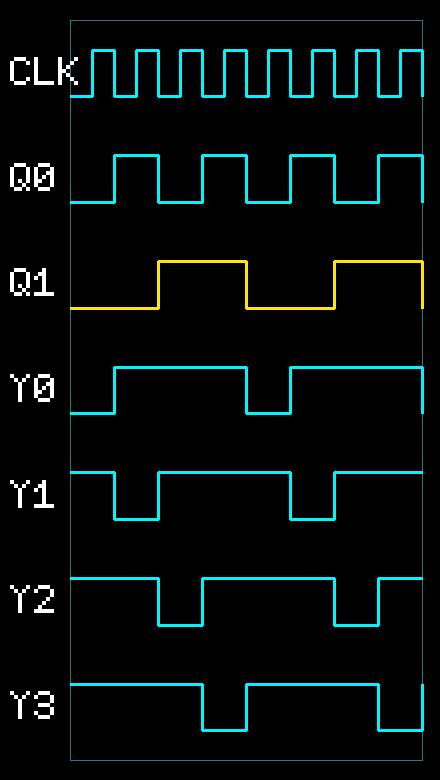
\includegraphics[width=0.95\textwidth]{figures/datas/E1/image7_waveform_replot.png}
    \caption{时序波形图}
\end{figure}

\section{实验总结}
本次实验完成了 74HC74 触发器功能验证、同步可逆模 4 计数器设计以及与非门译码器实现。实验结果表明，流水灯在 $M=0$ 与 $M=1$ 两种模式下均能按预期方向循环点亮，时序波形与理论分析一致。

本实验接线较复杂，实践中体会到“先模块化、后整体联调”的重要性。采用分块测试、逐点通断检查和示波器联合验证，可显著提升调试效率并降低故障定位难度。

\section{思考题}
\begin{enumerate}
    \item 为什么用 D 触发器也可以实现 T 触发器功能？

    解：因为 D 触发器满足 $Q_{n+1}=D$，令 $D=T\oplus Q_n$ 即可得到 $Q_{n+1}=T\oplus Q_n$，等效为 T 触发器。

    \item 本实验中为什么要把计数器与译码器分成两个模块？

    解：计数器负责“状态产生”，译码器负责“状态到输出映射”。模块分离便于推导、调试和故障定位，也利于后续扩展到更多位的流水灯系统。

    \item 若出现四个 LED 同时点亮，应优先检查哪些环节？

    解：应优先检查译码器连线是否错误、输出是否低有效接法混淆、供电与地线是否可靠，以及芯片是否存在损坏或接触不良。
\end{enumerate}

\end{document}
